\scanpage{70}
% archive sheet number: 69
% Several long oblique cancellation strokes cross the draft.
\deleted{\uline{Examples} 7.5.3. \mbox{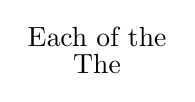
\begin{tikzpicture}[baseline=(base.base)]
\node[inner sep=0] (base) {\deleted{The}};
\node[anchor=south,inner sep=0,yshift=.08cm,xshift=0cm] at (base.north) {\inserted{Each of the}};
\end{tikzpicture}} following properties \raisebox{1.7ex}{\inserted{\uuline{R}}} satisfies the \mbox{
\begin{tikzpicture}[baseline=(word.base)]
\node[inner sep=0] (word) {condition};
\path (word.north west) -- coordinate[pos=.32] (mark) (word.north east);
% Isolated short brownish vertical trace; no letter or function assigned.
\draw[line width=.4pt] ([yshift=.08cm]mark) -- ([yshift=.21cm,xshift=-.01cm]mark);
\end{tikzpicture}} a) and b) of 7.5.1., \deleted{provided that $B$ is a} when $B$ is an excellent ring:}
\begin{enumerate}
\item[\deleted{(i)}] \deleted{$\operatorname{coprof}C\quad n$}
\item[\deleted{(ii)}] \deleted{$S_n$}
\item[\deleted{(iii)}] \deleted{Cohen--Macaulay}
\item[\deleted{(iv)}] \deleted{regular}
\item[\deleted{(v)}] \deleted{normal $R_n$}
\item[\deleted{(vi)}] \deleted{normal}
\item[\deleted{(vii)}] \deleted{integral}
\item[\deleted{(viii)}] \deleted{reduced}
\end{enumerate}

\deleted{In fact, for (vii) and (viii) this is true without any hypothesis on $B$, for (i) (ii) (iii) it suffices to \mbox{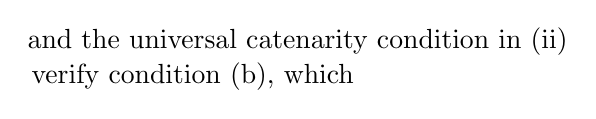
\begin{tikzpicture}[baseline=(base.base)]
\node[inner sep=0] (base) {verify condition (b), \deleted{which}};
\node[anchor=south west,inner sep=0,yshift=.08cm,xshift=-.05cm] at (base.north west) {\inserted{and the universal catenarity condition in (ii)}};
\end{tikzpicture}} that \mbox{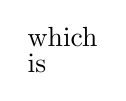
\begin{tikzpicture}[baseline=(base.base)]
\node[inner sep=0] (base) {is};
\node[anchor=south west,inner sep=0,yshift=.08cm,xshift=0cm] at (base.north west) {\inserted{which}};
\end{tikzpicture}} verified if \deleted{\unsure{all|so long} as} $B$ is a quotient of a regular ring, or satisfies Nagata's condition on the \mbox{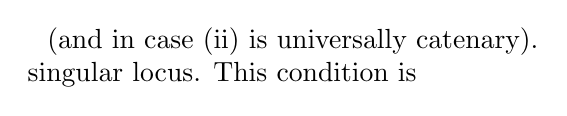
\begin{tikzpicture}[baseline=(base.base)]
\node[inner sep=0] (base) {singular locus. This condition is};
\node[anchor=south west,inner sep=0,yshift=.08cm,xshift=.25cm] at (base.north west) {\inserted{(and in case (ii) is universally catenary).}};
\end{tikzpicture}} also sufficient to make (iv) (v) (vi) work, provided that in (v) and (vi) one assumes in addition $B$ universally cate\rlap{h}nary. Finally, to make (vi) work, one can also take the condition ``$B$ is universally Japanese and universally catenary''.}
\margin{\deleted{\mbox{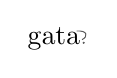
\begin{tikzpicture}[baseline=(word.base)]
\node[inner sep=0] (word) {gata};
% Faint extra curved impression and lower spot at the right of the last a; identity/function uncertain.
\draw[line width=.35pt,opacity=.65] ([xshift=-.05cm,yshift=.10cm]word.east) .. controls ([xshift=.09cm,yshift=.11cm]word.east) and ([xshift=.10cm,yshift=.03cm]word.east) .. ([xshift=.02cm,yshift=-.01cm]word.east);
\fill[opacity=.65] ([xshift=.04cm,yshift=-.05cm]word.east) circle (.015cm);
\end{tikzpicture}}}}

\deleted{\uline{Remarks} 7.5.4.\quad (i) as in 7.5.6. (i)}

\deleted{(ii) As in 7.5.6. (ii) ; it would in practice be a matter of the properties (i) \deleted{(ii)} (iii) (vii) or (viii).}

\deleted{(iii) In situation 7.5.1., one most often has an additional property of \uuline{R}, guaranteeing that if \deleted{$A\quad B$} $\text{\uuline{R}}(A)$ is true and the fibers of $\operatorname{Spec}(B)\quad\operatorname{Spec}(A)$ satisfy the geometric condition \uuline{R}, \deleted{the same is true} then \deleted{($\operatorname{Spec}(B)$ being} ($B$ being flat over $A$, let us recall) $\text{\uuline{R}}(B)$ is true. One can therefore de\rlap{e}duce from 7.5.1. that}
